\subsection{Reguladores paralelo}

Se dice que un regulador de tensión es paralelo cuando el elemento de control está en paralelo con la carga.\\
En la figura~\figref{fig:fig_parallel_regulator_example} se muestra un ejemplo, donde el elemento de control es un transistor. La operación del circuito es similar a la de un regulador serie, excepto porque la regulación se logra controlando la corriente a través de un transistor en paralelo, el cual deriva corriente.\\


\begin{figure}[H] %htb
\begin{center}
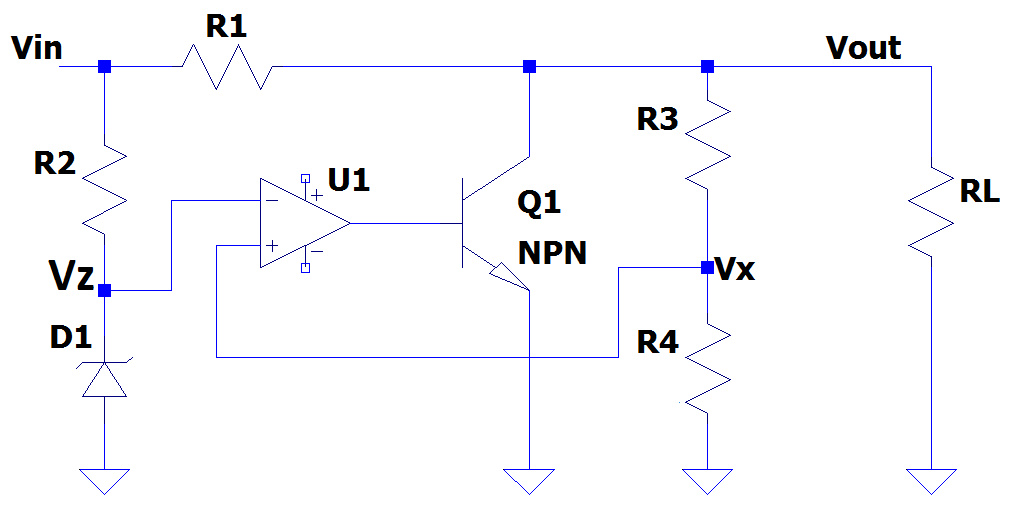
\includegraphics[width=0.6 \textwidth, angle=0]{./img/reguladores/parallel_regulator_example.png}
\caption{\label{fig:fig_parallel_regulator_example}\footnotesize{ejemplo de esquema de regulador paralelo}}
\end{center}
\end{figure}


Con $V_{(+)} = V_{(-)}$, tenemos :

\begin{equation*}
V_{z} = V_{in} - V_{R_{2}}
\end{equation*}

\begin{equation*}
V_{(-)} = V_{z}
\end{equation*}

\begin{equation*}
V_{(+)} = V_{out} \cdot  \frac{R_{4}}{R_{3} + R_{4}}
\end{equation*}


\begin{equation*}
\longrightarrow  V_{out} = V_{z} \left( 1 + \frac{R_{3}}{R_{4}} \right)
\end{equation*}



Un  cambio de la corriente de carga provoca un cambio opuesto de la corriente en paralelo.\\

\begin{equation*}
\Delta I_{c} = - \Delta I_{R_{L}}
\end{equation*}




Si el $V_{out}$ trata de reducirse, debido a la variación de la resistencia de la carga, $R_{3}$ y $R_{4}$ realimentan esta reducción, $V_{x}$ se reduce y excita menos a $Q_{1}$, la corriente en su colector se reduce y el voltaje se incrementa, este incremento compensa la reducción original del voltaje, y la salida se mantiene regulada. Análogamente ocurre si $V_{out}$ se incrementa.\\
Como ventaja vemos que el regulador paralelo tiene una protección contra cortocircuitos nativa debido a su configuración, y la corriente de la carga no circula por el elemento de regulación, y como desventaja, se disipa potencia en los elementos de regulación aunque no exista carga, y es proclive a sobre-tensiones en la carga, lo cual puede ser muy grave.








\clearpage